\setchapterpreamble[u]{\margintoc}
\chapter{Scenario Assessments -- Nuclear}
\labch{scenario_assessments}

In this chapter I will go over the physical limitations of 100\% Renewable scenarios, from pumped storage locations and scale to batteries materials mining and photovoltaic and wind land area constraints.

This section discusses the issues for nuclear, and for a mix

\section{Locations II -- Nuclear Siting}

Siting a nuclear power plant is a complex process. One needs to assess several physical characteristics, as well as societal ones.

\begin{itemize}
\item Seismic Risk
\item Landslide Risk
\item Flooding Risk
\item Protected Areas
\item Population Density
\item Water Access
\item Infrastructure Access
\end{itemize}

We want to be in a low-risk zone in term of natural hazards, in a region where the construction is possible (infrastructure access and right to build), and relatively close to water. At the same time, we'd like to be close to population centers to allow for more efficient electricity transport, while respecting guidance on exclusion zones. A lot of these societal parameters can vary, depending on the risk tolerance at a given location and the type of reactor considered.

When siting a power plant, especially a nuclear power plant, careful considerations must be taken into account. One of the most notable is the energy need. No sense in building a nuclear plant if there is no market for it within a reasonable distance.


\begin{figure*}
\begin{tabular}{cc}
  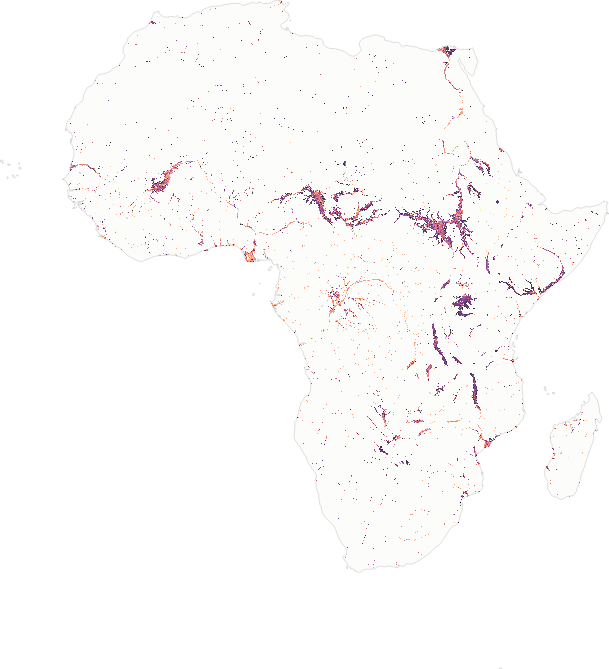
\includegraphics[width=50mm]{filter_flood} &   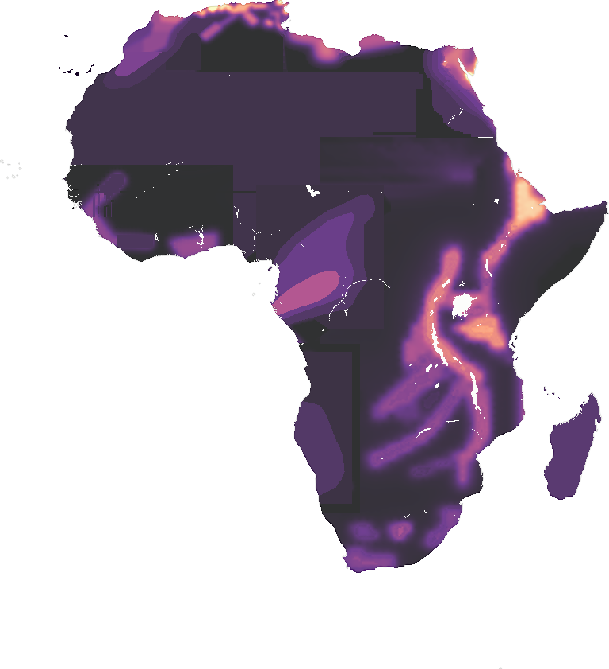
\includegraphics[width=50mm]{filter_pga} \\
(a) Flood & (b) Seismic \\[6pt]
 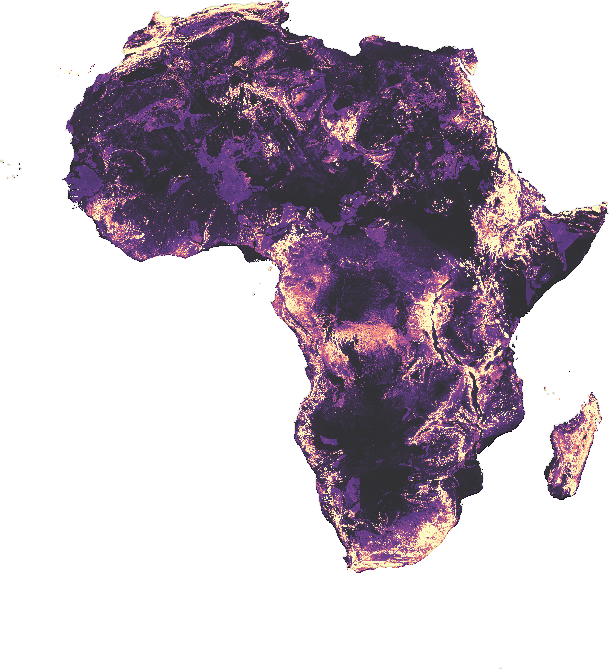
\includegraphics[width=50mm]{filter_landslides} &   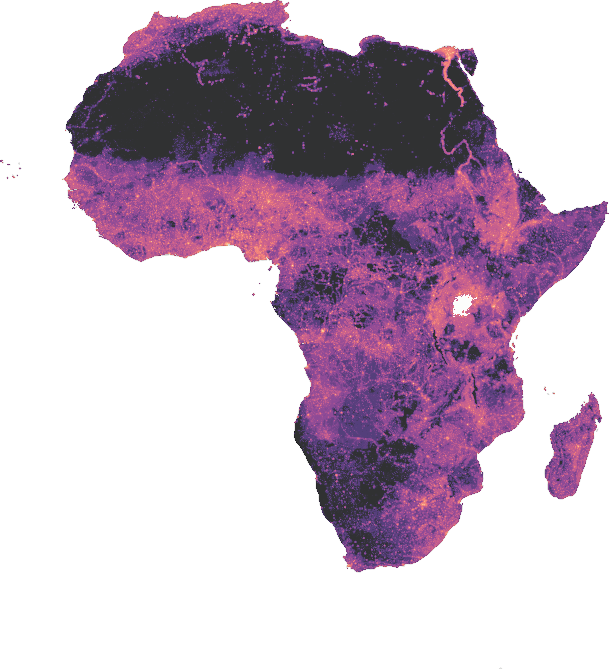
\includegraphics[width=50mm]{filter_population_r10mi} \\
(c) Landslides & (d) Population\\[6pt]
 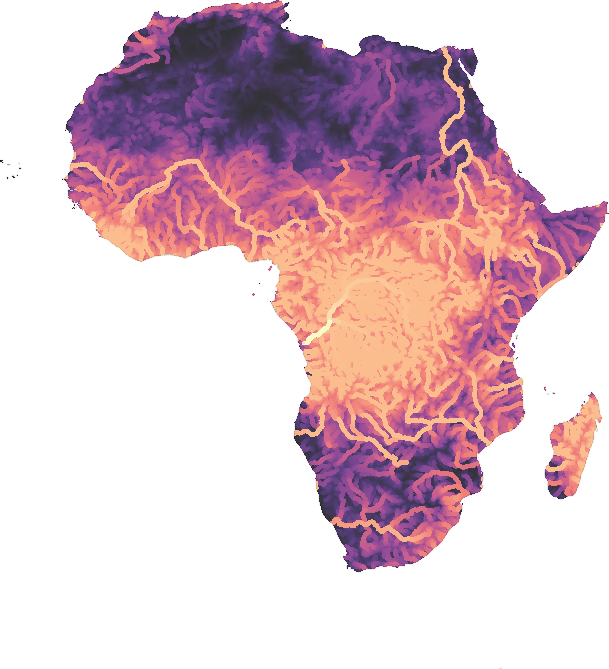
\includegraphics[width=50mm]{filter_rivers_maxqmin20mi} &   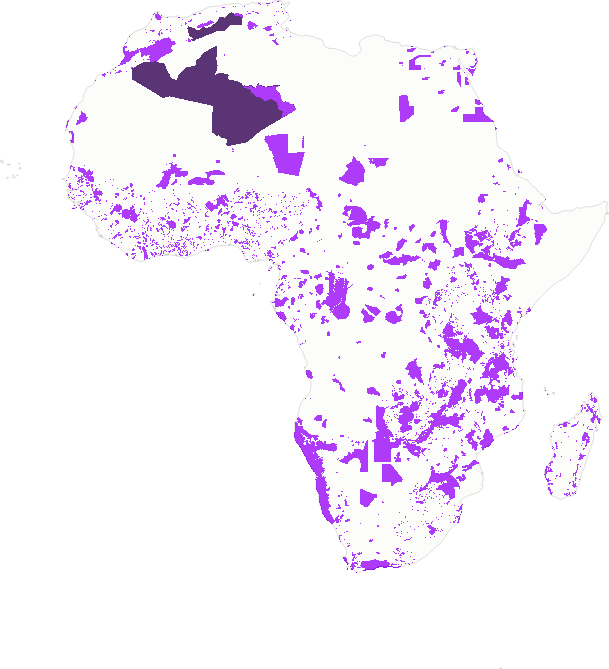
\includegraphics[width=50mm]{filter_protected} \\
(e) River Flows & (f) Protected Areas \\[6pt]
\end{tabular}
\caption{Filters for nuclear siting potential in Africa}
\labfig{nuclear_siting_filters}
\end{figure*}

Using the filters given in \vreffig{nuclear_siting_filters}, we can superimpose them and obtain a map of potential locations for Small Modular Reactors specifications and regulations.



\begin{figure}[h]
	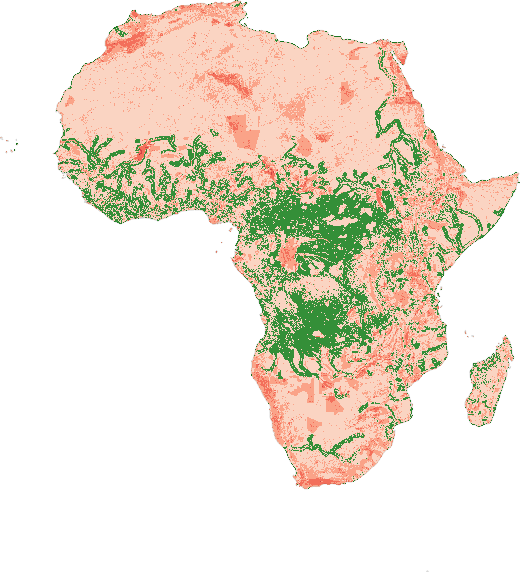
\includegraphics[width=1.0\textwidth]{filter_africa_lenientcase_nrc}
	\caption[Potential siting location (in green) and scale of unsuitable location (red shade) for regulation considerations. We can see that the green follows the river beds mostly. Water access is by far the limiting factor.]{Potential siting location (in green) and scale of unsuitable location (red shade) for regulation considerations. We can see that the green follows the river beds mostly. Water access is by far the limiting factor.}
	\labfig{filter_africa_lenientcase_nrc}
\end{figure}

\vreffig{filter_africa_lenientcase_nrc} shows that a large area of Africa is right away eliminated, mostly due to insufficient river flows. This is not per se surprising, and not an issue in and of itself, as people\sidenote[][-2mm]{And consequently energy needs} tend to live by the water. However, folding in considerations for existing infrastructure (roads or railways to transport construction materials and fuel supplies, or transmission lines network around to connect to the grid) severely changes the map, as shown in \vreffig{filter_africa_lenientcase_nrc_econ}. 10\% of the land in Africa is available in the first case, while it becomes only 1.5\% when existing infrastructure is accounted for.


\begin{figure}[h]
	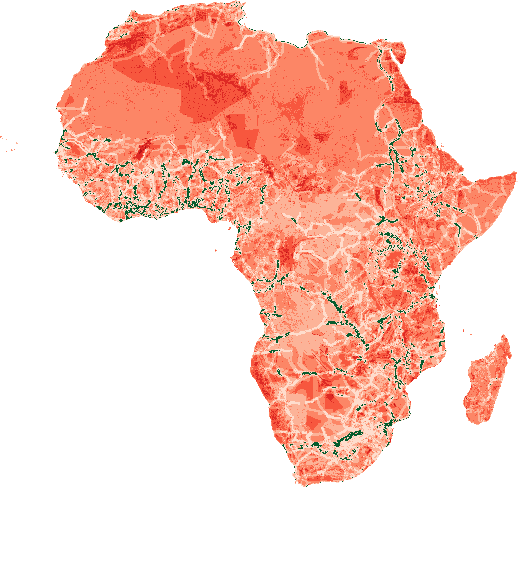
\includegraphics[width=1.0\textwidth]{filter_africa_lenientcase_nrc_econ}
	\caption[Potential siting location (in green) and scale of unsuitable location (red shade) for regulation and some economic considerations]{Potential siting location (in green) and scale of unsuitable location (red shade) for regulation and some economic considerations.}
	\labfig{filter_africa_lenientcase_nrc_econ}
\end{figure}

The density of nuclear energy allows for a small area to be necessary to power a large amount of people. Combined to this, the population center locations, combined with the needs for energy development, allows for this issue to be quite mitigated. The siting of nuclear reactor is however absolutely not to minimize, especially in developing and politically unstable countries, as we will touch on later on.

An issue not yet considered here is the potential future impact of droughts, made more frequent by climate change, on water supplies. Only historical droughts are accounted for. This can very negatively impact the operation of nuclear power plants, which may have to be offline for extended period of time due to a lack of cooling water.

\section{Materials V -- Uranium}

Uranium resources are not plentiful despite the punch it can pack~\sidecite{grancea2020uranium}. Available resources are often separated by estimated cost of access, ranging from less than \$40 per kilogram to more than \$260 per kilogram. This gives an estimated reserves between 2.2 and 16 MT.

This severely limits the viability of nuclear on the long term. France alone, going 100\% nuclear for the next century, would need around 2.4 MT.

But, there are silver linings:

\begin{itemize}
\item Fuel recycling: We can, and some countries have had successful recycling programs, which can save up to X\% of the uranium need.
\item Thorium: Nuclear can also work using the Thorium nuclides chain. Thorium is about three times as plentiful as Nuclear.
\item Current reactor technologies use the u-235 isotope of uranium, which occurs at a concentration of 0.7\%. We have since developed advanced reactor which can use natural uranium directly\sidenote[][-2mm]{Several such reactors were tested at scale and even used in actual production, notably in France. They are called breeder because they can transform the 99.7\% fraction of uranium that is $\mathrm{U_238}$ into fissile plutonium, and burn it in a cycle.}.
\end{itemize}

Things are not as simple as simply moving to the advanced reactors however, and it is important to keep that in mind. There are concerns over plutonium proliferation (weapons) in the use of breeder reactors, and there are still many hurdles to overcome to be able to deploy them efficiently at scale.

Removing the recycling ban on nuclear fuel in multiple countries, such as the USA, would go a long way toward buying time.

\blindtext

\section{Public Opinion}

Public opinion is difficult to change quickly and react strongly to fear

\blindtext

\section{Waste}

Waste is an issue, but not a big one. Appendix: Hopes from Oklo

\blindtext

\section{Timeline}

Nuclear takes time to develop, while renewable are fast.

\blindtext

\section{Economical mix}

Renewable need to be super cheap to compete with nuclear fuel generation in today's market, or policies will need to be created to account for this

\blindtext



\section{The Digest}

\begin{kaoboxgreen}[frametitle=Main Takeaways]

\begin{itemize}
\item The \emph{finite materials problem} is very real and is an unmovable wall in the way of 100\% renewable scenarios.
\item Renewable energy is indeed renewable by definition, but capturing that energy is not renewable.
\item Building up energy storage systems or wind turbines use up either finite geographical locations or finite materials resources at an alarming and absolutely not sustainable rate.
\item Recycling will have to become prevalent for some materials. It will not be enough to cover the needs of a 100\% renewable system, but still absolutely needs to be developed.
\end{itemize}
  
\end{kaoboxgreen}